%!TEX root = ../../super_main.tex
\chapter{Introduction}
\label{cha:introduction}

%Technology can enhance the quality of our lives in many different ways. A new airbag technology in our cars or an intelligent thermostat in our house. New technology helps us on many different aspects. These technologies also includes software, that enables devices to assist people in new and innovative ways.
%\\\\
% Purpose of software
This report focuses on the continued development of an existing \emph{Android}-software suite for tablets called \giraf (Graphical Interface Resources for Autistic Folk), which includes tools and games to assist and train everyday aspects of life for citizens diagnosed an Autism Spectrum Disorder (ASD) \parencite{asd}. The tool is currently in development but should, when finished, be used as an digital alternative to the already existing tools and techniques used \parencite{birken_slides}.
\\\\
This system has three types of users, the citizens diagnosed with ASD and the institutional or legal guardians of these citizens. The last type of users is the administrators. Using \giraf, a citizen can find tools to mimic and learn social patterns\todo{Mention how the application help citizens with spoken language}. The guardians customize the various application such that they are optimized for the needs of the individual citizens. \todo{Write something about the administers. What are they supposed to do in the regards to the system?}
\\\\
The primary customer of \giraf is the municipality of Aalborg, where one of the main stakeholders of the \giraf-system is a kindergarten called \emph{Birken}. This kindergarten takes care of children diagnosed with ASD. The staff in \emph{Birken} spend a lot of time preparing physical and visual weekly schedules and checklists based on laminated printouts for the children which helps with their daily functions. This has motivated some of the previous developers of the \giraf project to try to digitize the schedule and checklists currently used. \todo{Insert reference to birken somewhere in this section}

%!TEX root = ../../super_main.tex

\section{Multi project organization}

This semester project is the continuation of a widely spanning multi project with 52 developers which are organized in 14 smaller groups, up to four developers per group, including a group consisting of the authors of this report. The multi project was split into 3 different project areas: Build and Deployment, GUI, Database. 

\subsection{Organization}
The multi project was organized using the development method Scrum\parencite{scrum}, more specific Scrum of Scrums. This method alows the multiproject to be self-organized and enforces the individual groups to do work more independetly. This independent work fits great in since the individual groups is used to work in smaller projects groups. However in this semetester the groups will now obtain experience in working on a larger scale projects than previous encountered in their education. 
\\\\
As seen in \figref{fig:scrum_of_scrums} the Scrum of Scrums is split into three levels. The bottom most level is the individual groups, which work exactly as an ordinary development group using the Scrum method. The middle layer contains the three project areas where representatives from each individual group meet and syncronize their work at least twice a week. The top layer in \figref{fig:scrum_of_scrums} contains representatives from all of the project areas. However since standup meeting only occur once a week in this Scrum representatives from all groups are encouraged to join the meetings.

\todo[inline]{Update Figure}
\begin{figure}[!htbp]
  \centering
    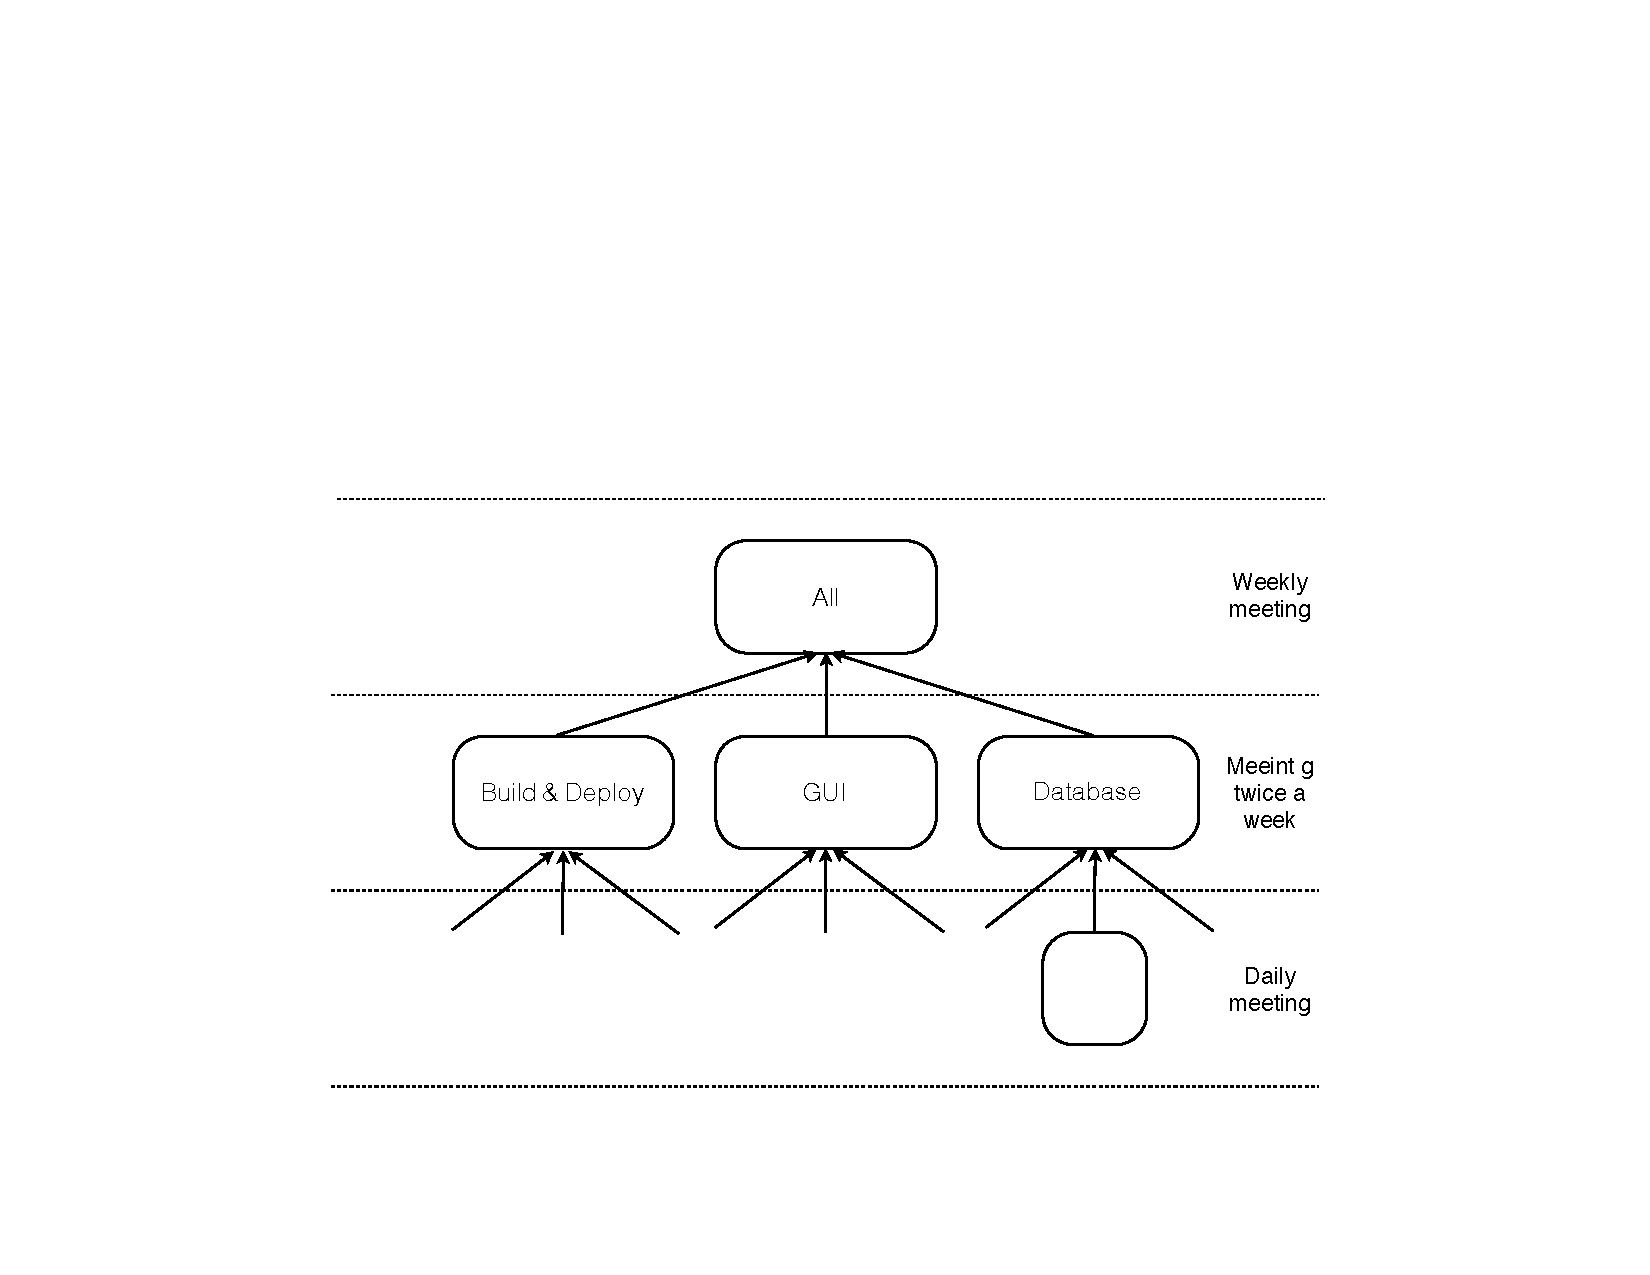
\includegraphics[width=0.6\textwidth]{scrum_of_scrums}
    \caption{Organization in Scrum of Scrums.}
    \label{fig:scrum_of_scrums}
\end{figure}



\subsection{Roles and Responsibilities}
Several different roles and responsibilities were divided among the project groups. This group volunteered as ``Webadmin'' and also included an Android Guru.

The ``Webadmin'' responsibility included administration of the official \giraf web page. 

